\section{Вычислительный эксперимент}\label{sec4}

Проводится эксперимент для анализа свойств предложенных методов оценки достаточного размера выборки. Эксперимент состоит из нескольких частей. В первой части рассматриваются оценки достаточного размера выборки в случае, когда достаточный размер выборки не превосходит доступный. Во второй части исследуются результаты, полученные в условиях того, что достаточный размер выборки больше доступного.

\subsection{Достаточный размер выборки не превосходит доступный}

\subsubsection{Бутстрапирование функции правдоподобия}

\paragraph{Сходимость функций $D(k)$ и $M(k)$.}

Синтетические данные сгенерированы из моделей линейной и логистической регрессий. Число объектов 1000, число признаков 20. Используется $B=1000$ бустрапированных подвыборок. Подсчитываются значения функций $D(k)$ и $M(k)$. Датасет с задачей регрессии Liver Disorders из \cite{UCI} содержит 345 объектов и 5 признаков. Мы также используем $B=1000$ бутстрапированных подвыборок для оценки математического ожидания и дисперсии функции ошибки.

На Рис.~\ref{likelihood-synthetic-regression} можно видеть полученные зависимости между используемым размером подвыборки $k$ и рассматриваемыми функциями $D(k)$ и $M(k)$ для синтетической выборки с задачей регрессии. Результаты для синтетической выборки с задачей классификации представлены на Рис.~\ref{likelihood-synthetic-classification}. В то же время, на Рис.~\ref{likelihood-liver-disorders} мы видим аналогичные графики для датасета Liver Disorders. Видно, что во всех случаях значения функций $D(k)$ и $M(k)$ стремятся к нулю при увеличении размера выборки. Эти эмпирические результаты подтверждают теоретические, полученные ранее.

\begin{figure}[h!]
    \centering
    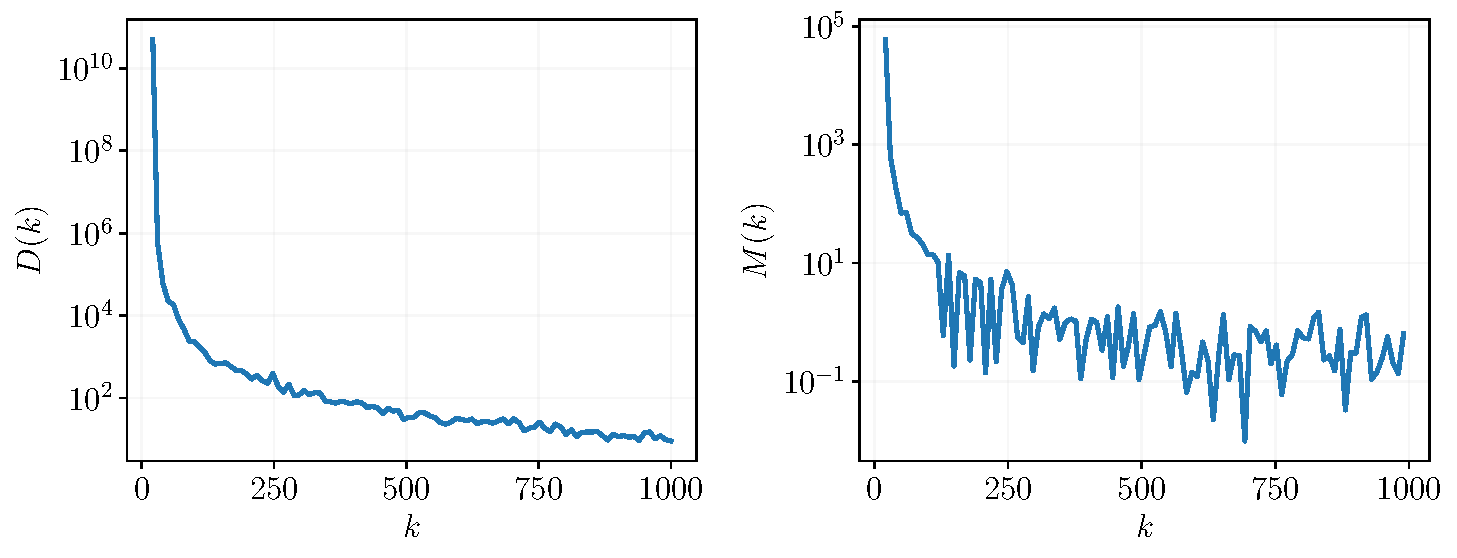
\includegraphics[width=\textwidth]{likelihood-synthetic-regression}
    \caption{Синтетическая выборка (линейная регрессия)}
    \label{likelihood-synthetic-regression}
\end{figure}

\begin{figure}[h!]
    \centering
    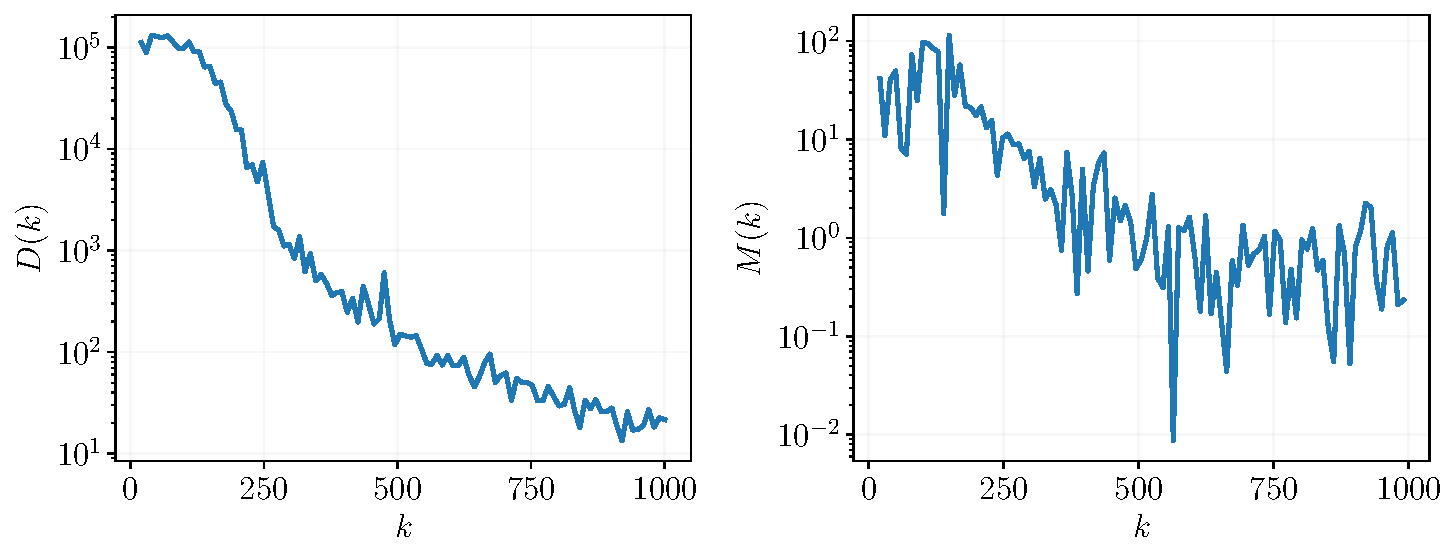
\includegraphics[width=\textwidth]{likelihood-synthetic-classification}
    \caption{Синтетическая выборка (логистическая регрессия)}
    \label{likelihood-synthetic-classification}
\end{figure}

\begin{figure}[h!]
    \centering
    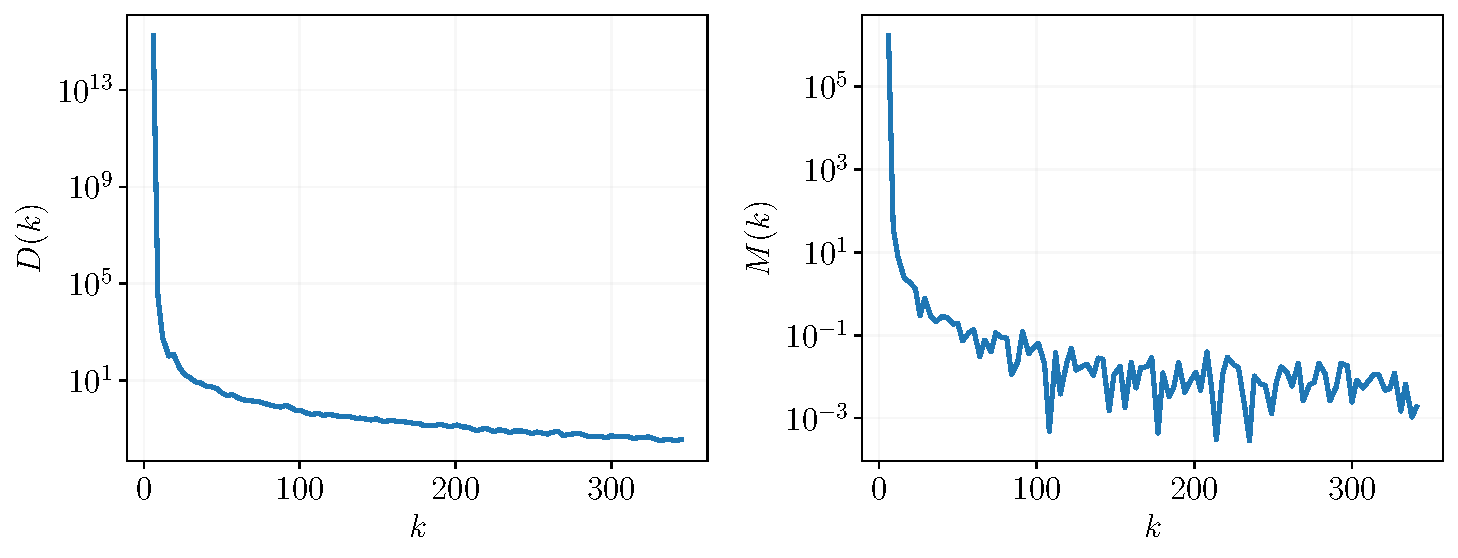
\includegraphics[width=\textwidth]{likelihood-liver-disorders}
    \caption{Выборка Liver Disorders (регрессия)}
    \label{likelihood-liver-disorders}
\end{figure}

\paragraph{Варьирование гиперпараметра $\varepsilon$ для достаточного размера выборки.}

В определениях D-достаточности и M-достаточности участвует гиперпараметр $\varepsilon$, который отвечает за порог для достаточного размера выборки $m^*$. С целью изучения зависимости между ними, мы представляем Рис.~\ref{likelihood-sufficient-vs-threshold}, который демонстрирует, какой размер выборки следует выбрать, чтобы обеспечить определенный уровень уверенности.

\begin{figure}[h!]
    \centering
    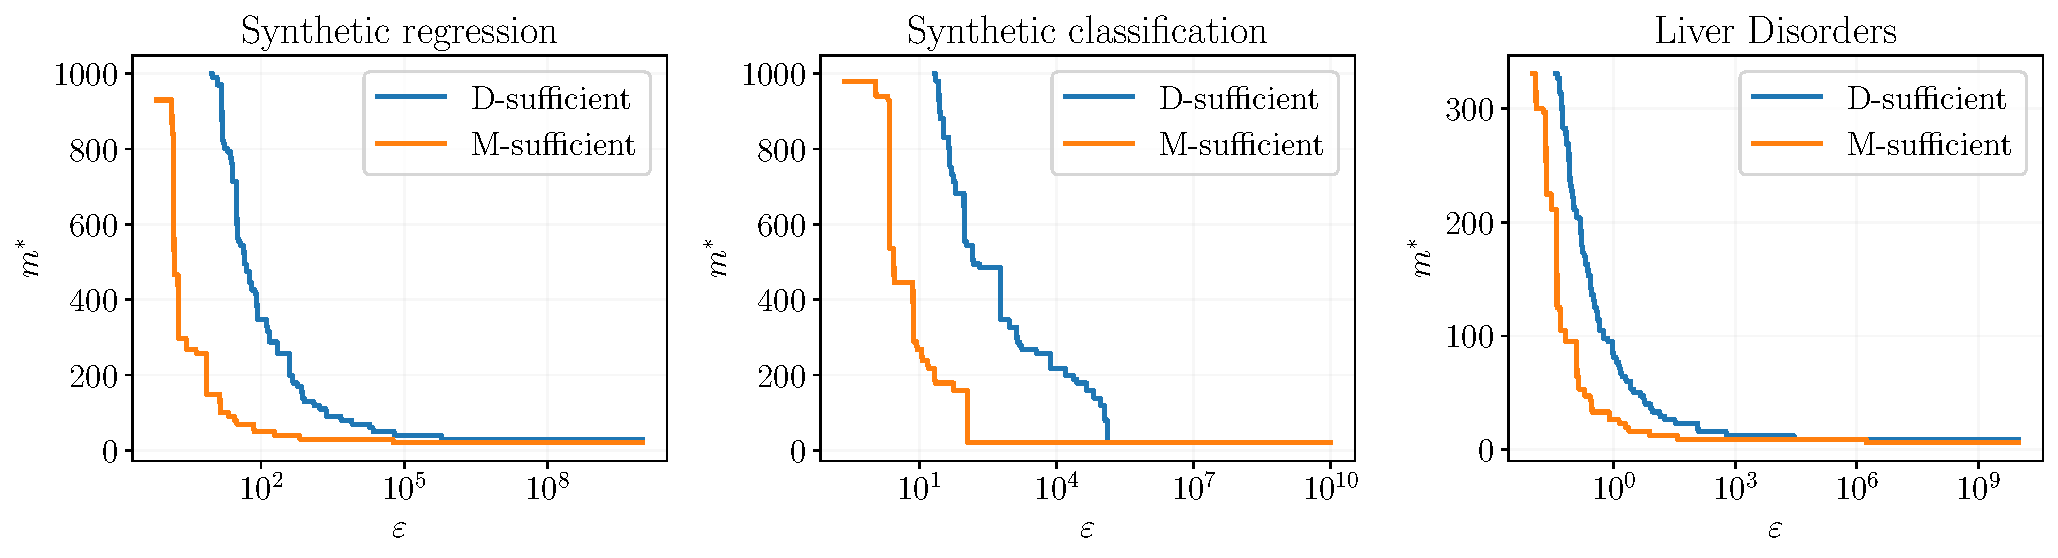
\includegraphics[width=\textwidth]{likelihood-sufficient-vs-threshold}
    \caption{Достаточный размер выборки в зависимости от гиперпараметра $\varepsilon$}
    \label{likelihood-sufficient-vs-threshold}
\end{figure}

\subsubsection{Близость апостериорных распределений}

\paragraph{Сходимость апостериорных распределений.}

Используется синтетическая выборка, сгенерированная из модели линейной регрессии. С целью упрощения визуализации рассматриваются одномерный и двумерный случаи. Число объектов 100, среднеквадратичное отклонение шума 1, априорное распределение параметров $\mathcal{N}(\bw | \mathbf{0}, \bI)$. Далее представлены Рис.~\ref{posterior-1d-similarity} и Рис.~\ref{posterior-2d-similarity}, на которых изображено сходство апостериорных распределений, определенных на схожих подвыборках размера $k$ и $k+1$.

\begin{figure}[h!]
    \centering
    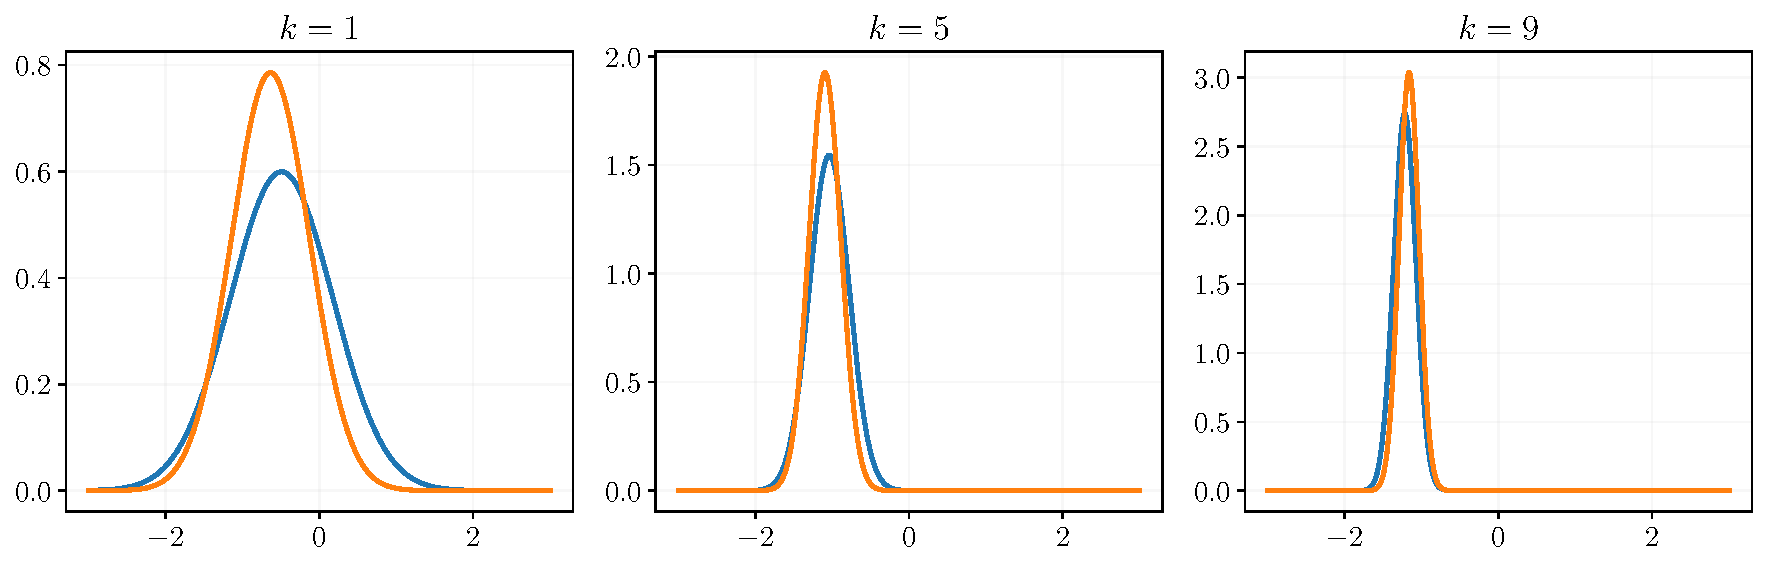
\includegraphics[width=\textwidth]{posterior-1d-similarity}
    \caption{Апостериорные распределения параметров на схожих подвыборках (одномерный случай~--- графики плотностей распределения)}
    \label{posterior-1d-similarity}
\end{figure}

\begin{figure}[h!]
    \centering
    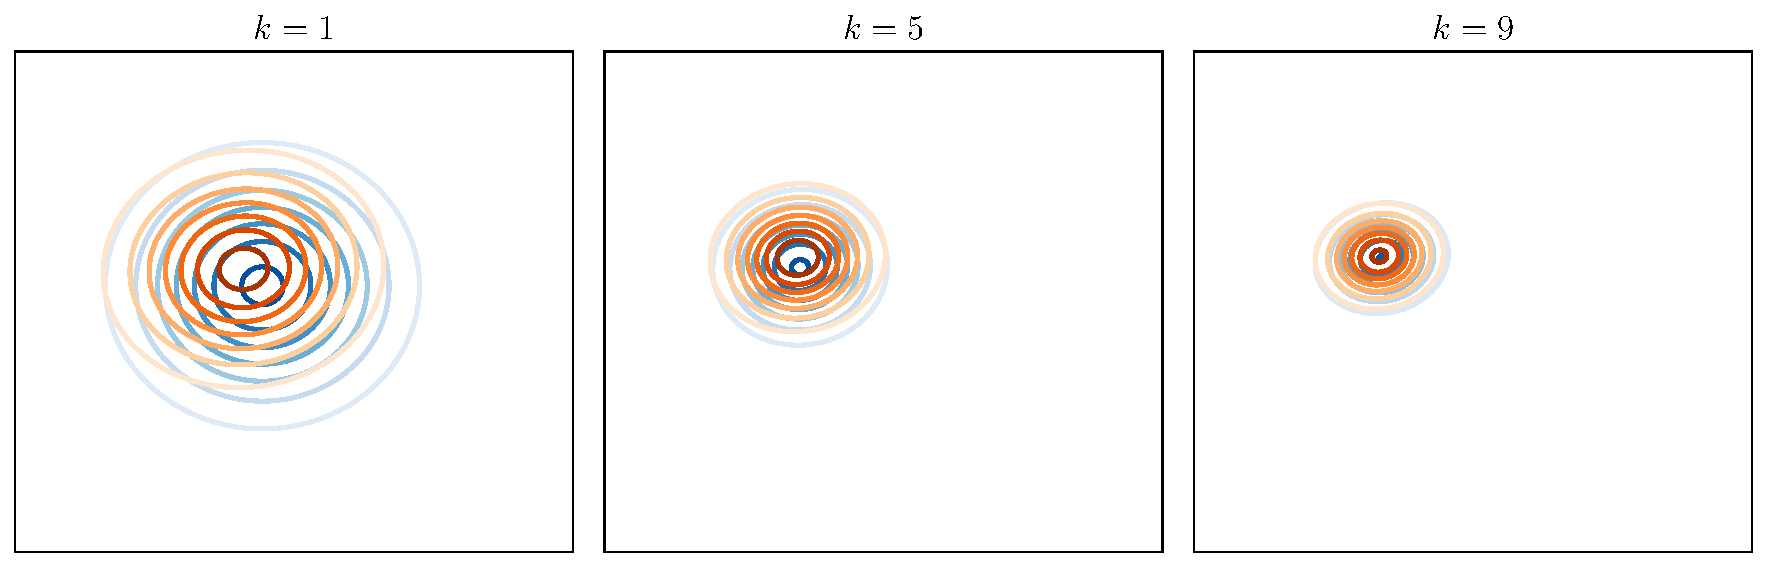
\includegraphics[width=\textwidth]{posterior-2d-similarity}
    \caption{Апостериорные распределения параметров на схожих подвыборках (двумерный случай~--- графики линий уровня)}
    \label{posterior-2d-similarity}
\end{figure}

Видно, что в обоих случаях распределение параметров становится схожим при росте доступного размера выборки. Эта интуиция и послужила фундаментом для предложенных в настоящей работе методов.

\paragraph{Асимптотическое поведение минимального собственного значения матрицы $\bX\T\bX$.}

Синтетические данные сгенерированы из модели линейной регрессии. Число объектов 500, число признаков 10. Один объект последовательно удаляется из данной выборки, пока число объектов в подвыборке не станет равно числу признаков. Для каждого размера выборки $k$ подсчитывается минимальное собственное значение матрицы $\mathbf{X}_k\T \mathbf{X}_k$. Кроме того, подсчитываются значения функций $KL(k)$ и $S(k)$. Такой процесс повторяется $B=100$ раз.

Датасет с задачей регрессии Liver Disorders из \cite{UCI} имеет 345 объектов и 5 признаков. Мы аналогично удаляем объекты из выборки один за другим. Подсчитываются минимальное собственное значение и значения функций. Процесс повторяется $B=1000$ раз.

Рис.~\ref{posterior-eigvals} показывает асимптотическое поведение минимального собственного значения матрицы $\mathbf{X}_k\T \mathbf{X}_k$. Видно, что при стремлении размера выборки к бесконечности минимальное собственное значение также стремится к бесконечности. Помимо этого, как и требуется в Теореме~\ref{theorem4}, этот график лежит выше, чем $\sqrt{k}$.

\begin{figure}[h!]
    \centering
    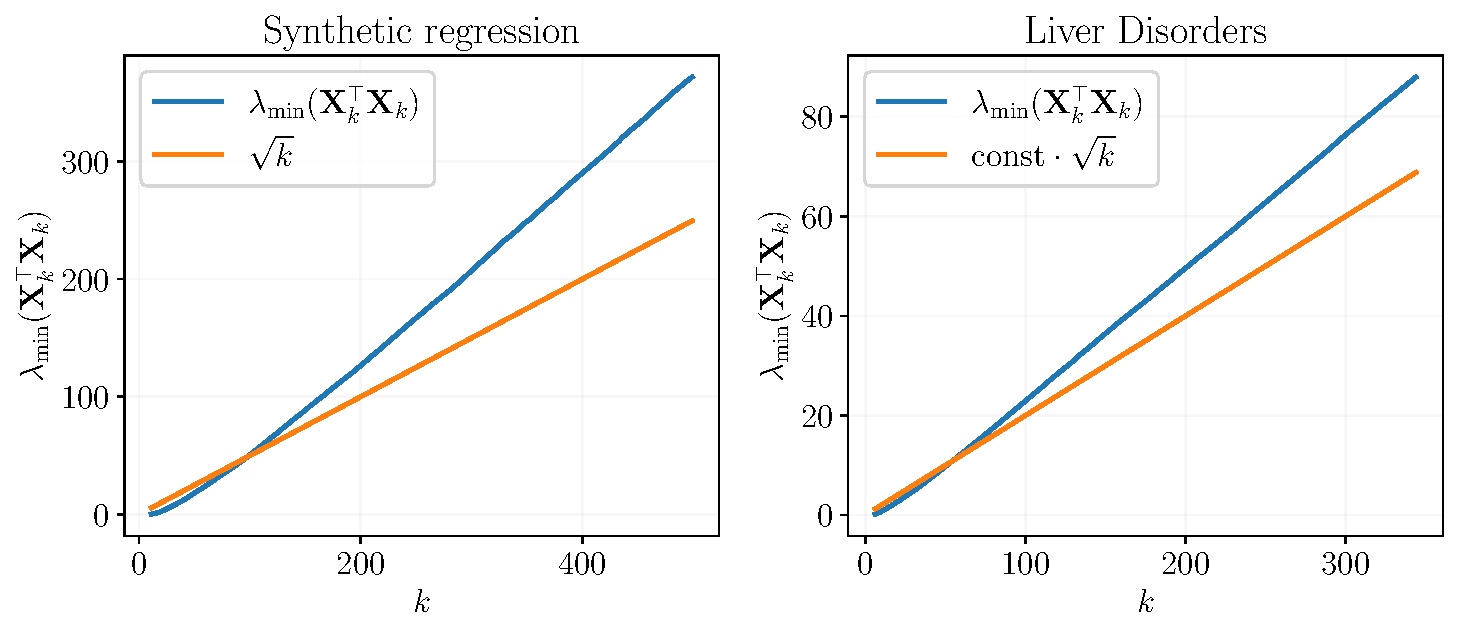
\includegraphics[width=\textwidth]{posterior-eigvals}
    \caption{Минимальное собственное значение матрицы $\mathbf{X}_k\T \mathbf{X}_k$}
    \label{posterior-eigvals}
\end{figure}

\paragraph{Сходимость функций $KL(k)$ и $S(k)$.}

На Рис.~\ref{posterior-synthetic-regression} мы можем наблюдать полученные зависимости между доступным размером выборки $k$ и предложенными функциями $KL(k)$ и $S(k)$ для синтетической выборки с задачей регрессии. В то же время, на Рис.~\ref{posterior-liver-disorders} можно видеть аналогичные графики для датасета Liver Disorders. Для обеих выборок значения функции $KL(k)$ стремятся к нулю при увеличении размера выборки, а значения $S(k)$ стремятся к единице. Эти эмпирические результаты подтверждают теоретические, представленные ранее.

\begin{figure}[h!]
    \centering
    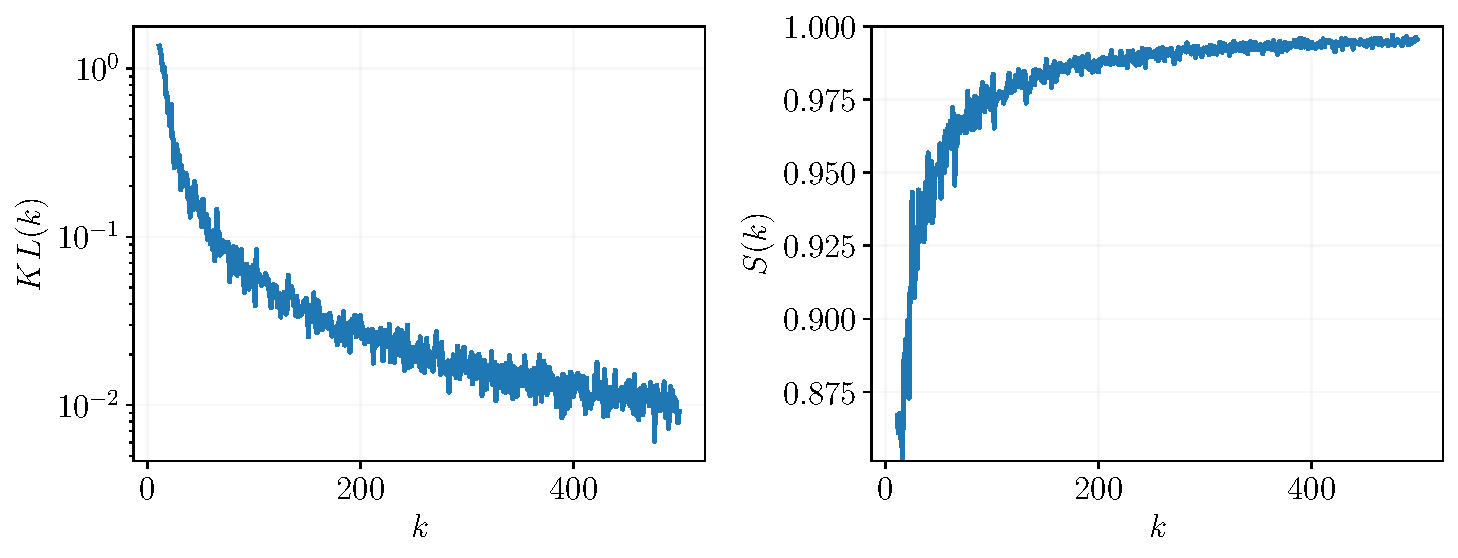
\includegraphics[width=\textwidth]{posterior-synthetic-regression}
    \caption{Синтетическая выборка (линейная регрессия)}
    \label{posterior-synthetic-regression}
\end{figure}

\begin{figure}[h!]
    \centering
    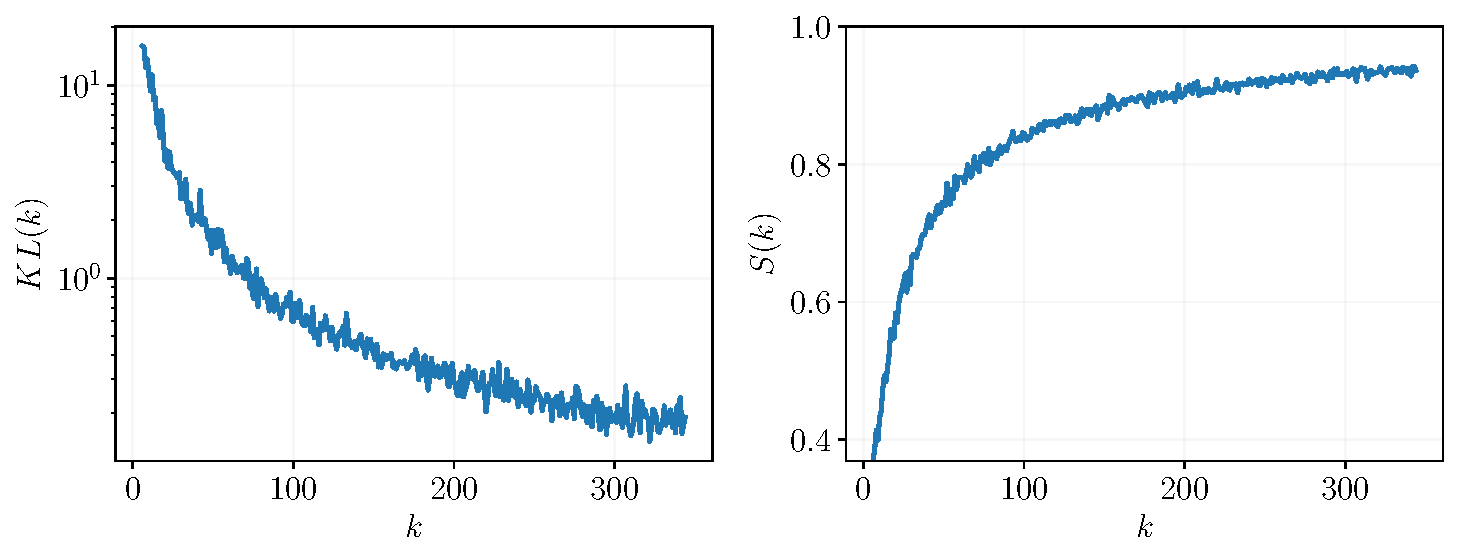
\includegraphics[width=\textwidth]{posterior-liver-disorders}
    \caption{Выборка Liver Disorders (регрессия)}
    \label{posterior-liver-disorders}
\end{figure}

\paragraph{Варьирование гиперпараметра $\varepsilon$ для достаточного размера выборки.}

В определениях KL-достаточности и S-достаточности участвует гиперпараметр $\varepsilon$, который отвечает за порог для достаточного размера выборки $m^*$. С целью изучения зависимости между ними, мы представляем Рис.~\ref{posterior-sufficient-vs-threshold}, который демонстрирует, какой размер выборки следует выбрать, чтобы обеспечить определенный уровень уверенности.

\begin{figure}[h!]
    \centering
    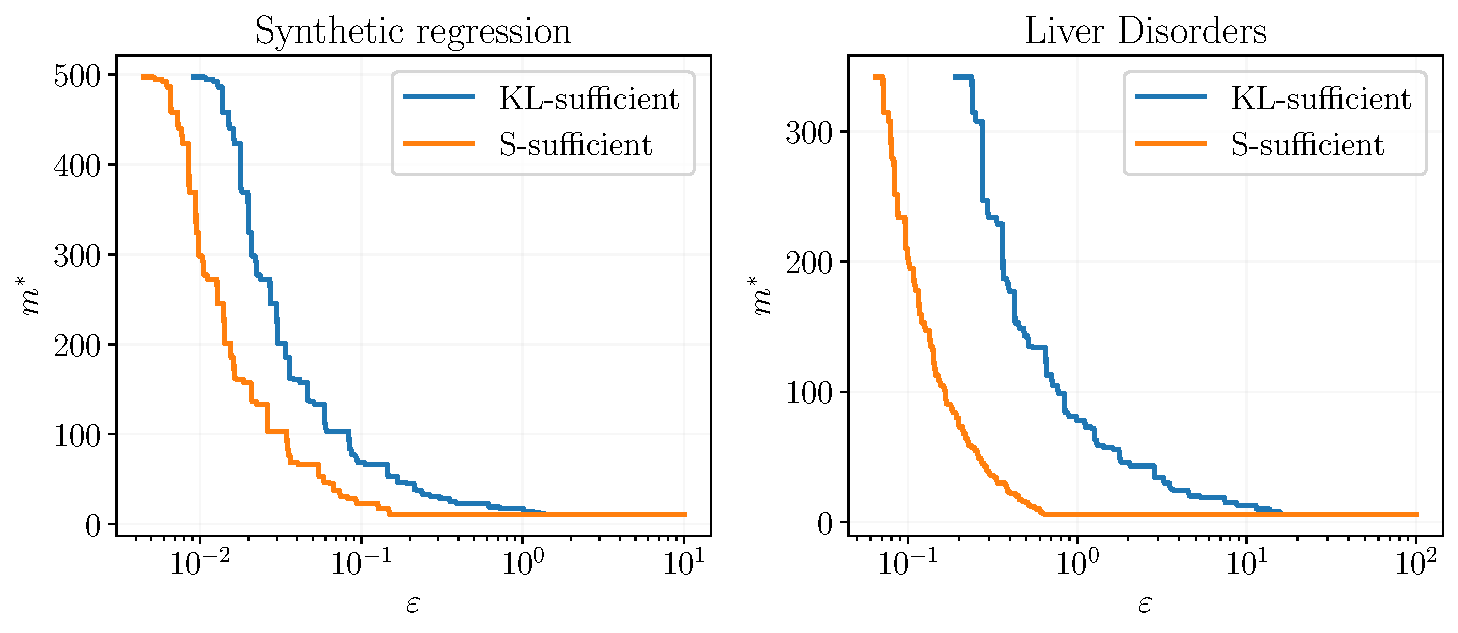
\includegraphics[width=\textwidth]{posterior-sufficient-vs-threshold}
    \caption{Достаточный размер выборки в зависимости от гиперпараметра $\varepsilon$}
    \label{posterior-sufficient-vs-threshold}
\end{figure}

Для $\varepsilon=10$ достаточно взять число объектов, равное числу признаков. Однако для $\varepsilon=10^{-2}$ требуется взять всю выборку.

\paragraph{Сравнение подходов на множестве выборок.}

Чтобы оценить эффективность предложенных методов на разных наборах данных, были выбраны выборки из открытой библиотеки \cite{UCI}. Подробная информация о каждом наборе данных, количество наблюдений и количество признаков представлены в таблице~\ref{table}. Для демонстрационных целей было выбрано значение гиперпараметра $\varepsilon$, при котором значение целевой функции $KL(k)$ или $S(k)$ уменьшается вдвое. Соответствующие результаты приведены в таблице~\ref{table}. Пропуски означают, что первоначальный размер выборки недостаточен.

\begin{table}
    \centering
    \caption{Выборки с задачей регрессии (пропуски означают, что первоначальный размер выборки недостаточен)}\label{table}
    \begin{tabular}{|c|c|c|c|c|}
    \hline
    Название выборки & Объектов $m$ & Признаков $n$ & KL & S \\
    \hline
    Abalone & 4177 & 8 & 3751 & 3751\\
    Auto MPG & 392 & 8 & 55 & --- \\
    Automobile & 159 & 25 & 152 & --- \\
    Liver Disorders & 345 & 6 & 282 & --- \\
    Servo & 167 & 4 & 138 & 160 \\
    Forest fires & 517 & 12 & 487 & --- \\
    Wine Quality & 6497 & 12 & --- & --- \\
    Energy Efficiency & 768 & 9 & --- & --- \\
    Student Performance & 649 & 32 & --- & --- \\
    Facebook Metrics & 495 & 18 & 379 & 475  \\
    Real Estate Valuation & 414 & 7 & --- & --- \\
    Heart Failure Clinical Records & 299 & 12 & 258 & 293 \\
    Bone marrow transplant: children & 142 & 36 & 109 & --- \\
    \hline
    \end{tabular}
\end{table}

%%% ЭТА ЧАСТЬ НАХОДИТСЯ В РАЗРАБОТКЕ
%%% ПОКА ЧТО ОЧЕНЬ СЫРОЙ МАТЕРИАЛ
\clearpage
\subsection{Достаточный размер выборки больше доступного}

\subsubsection{Определение параметрического семейства функций с помощью генетического алгоритма}

Реализацию генетического алгоритма, приведенного в разделе \ref{ga}, можно найти в \href{https://github.com/kisnikser/Bayesian-Sample-Size-Estimation/tree/main/code/genetic_algorithm}{репозитории}. Для исследования зависимости функции ошибки от используемого размера выборки в задаче регрессии использовались следующие датасеты из \citep{UCI}: Abalone, Auto MPG, Liver Disorders, Wine Quality, Parkinsons Telemonitoring, Bike Sharing Dataset, Real estate valuation и Heart failure clinical records. Была выбрана квадратичная функция потерь MSE. Задача регрессии для каждого из них решалась с помощью линейной регрессии из \citep{scikit-learn}. Усреднение производилось по $B = 100$ бутстрап-выборкам. Как было сказано ранее, все зависимости приводятся к одинаковому масштабу по обеим осям. Полученные графики представлены на Рис.~\ref{datasets-regression}. Слева находится график для выборочного среднего. Справа находится график для выборочного среднеквадратичного отклонения.

\begin{figure}[h!]
    \centering
    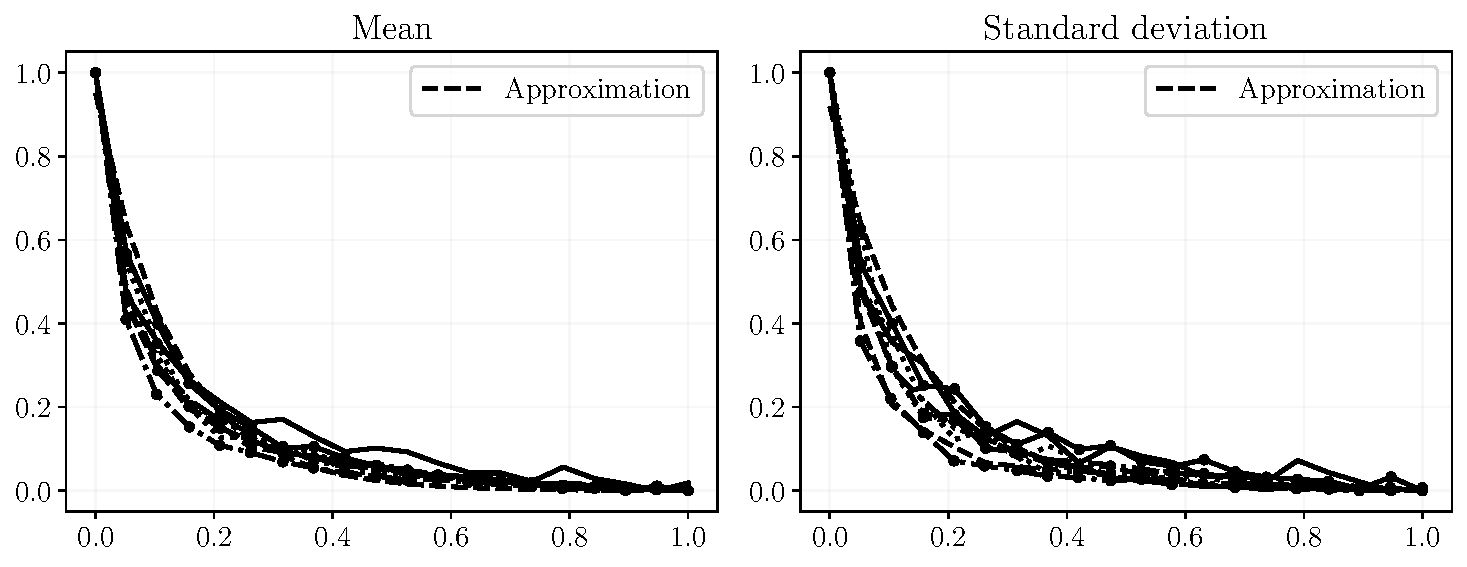
\includegraphics[width=\textwidth]{datasets-regression}
    \caption{Поведение функции ошибки в задаче регрессии}
    \label{datasets-regression}
\end{figure}

Применение генетического алгоритма приводит к одинаковому семейству функций для аппроксимации среднего и среднеквадратичного отклонения в задаче регрессии:
\[ w_0 + w_1 \cdot \exp(w_2 \cdot x). \]

В задаче классификации использовалось 12 датасетов из \citep{UCI}: Automobile, Breast Cancer Wisconsin (Diagnostic), Car Evaluation, Credit Approval, Glass Identification, Ionosphere, Iris, Tic-Tac-Toe Endgame, Congressional Voting Records, Wine, Zoo и Heart failure clinical records. Задача классификации для каждого из них решалась с помощью логистической регрессии из \citep{scikit-learn}. Усреднение производилось по $B = 100$ бутстрап-выборкам. Все завимисости также приводятся к одинаковому масштабу по обеим осям. Полученные графики представлены на Рис.~\ref{datasets-classification}. Как и ранее, слева находится график для выборочного среднего, справа находится график для выборочного среднеквадратичного отклонения.

\begin{figure}[h!]
    \centering
    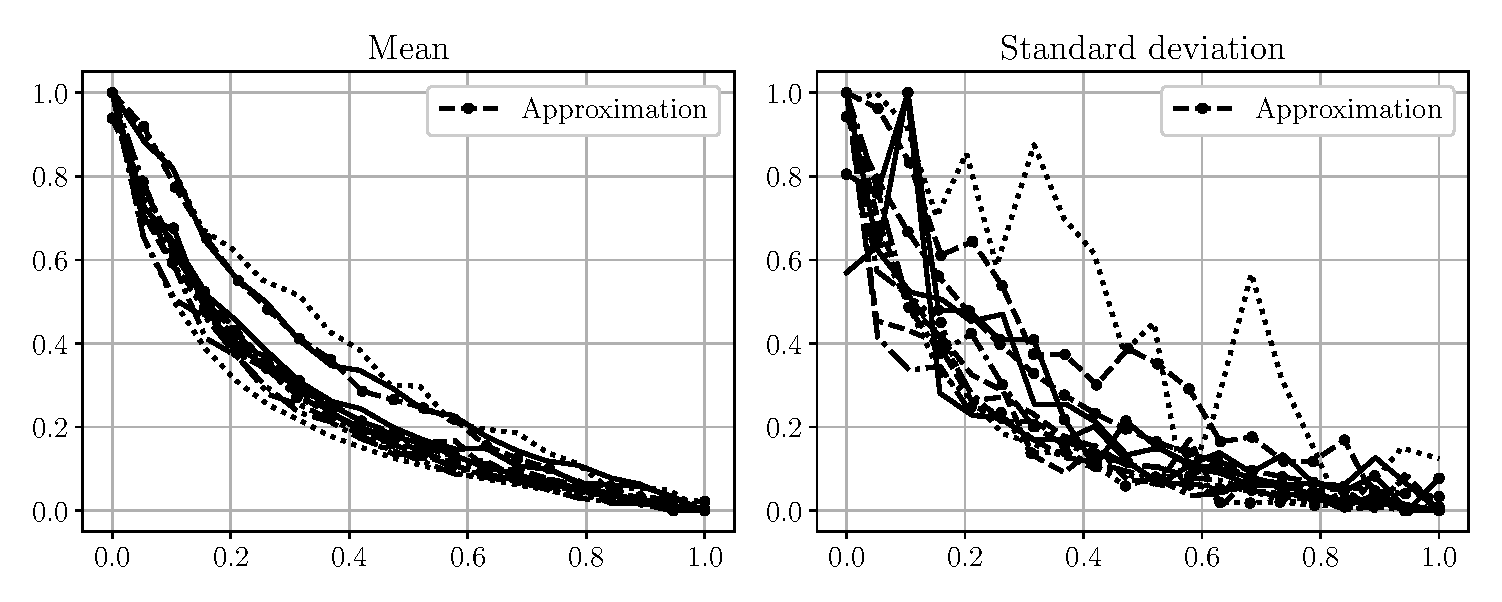
\includegraphics[width=\textwidth]{datasets-classification}
    \caption{Поведение функции ошибки в задаче классификации}
    \label{datasets-classification}
\end{figure}

Применение генетического алгоритма для среднего значения приводит к такому же семейству функций, как и в задаче регрессии:
\[ w_0 + w_1 \cdot \exp(w_2 \cdot x). \]

Среднеквадратичное отклонение в случае задачи классификации для каждой выборки имеет свою зависимость от размера выборки. Таким образом, прогнозировать дисперсию для классификации оказывается достаточно сложной задачей.

